%package list
\documentclass{article}
\usepackage[top=3cm, bottom=3cm, outer=3cm, inner=3cm]{geometry}
\usepackage{multicol}
\usepackage{graphicx}
\usepackage{url}
%\usepackage{cite}
\usepackage{hyperref}
\usepackage{array}
%\usepackage{multicol}
\newcolumntype{x}[1]{>{\centering\arraybackslash\hspace{0pt}}p{#1}}
\usepackage{natbib}
\usepackage{pdfpages}
\usepackage{multirow}
\usepackage[normalem]{ulem}
\useunder{\uline}{\ul}{}
\usepackage{svg}
\usepackage{xcolor}
\usepackage{listings}
\lstdefinestyle{ascii-tree}{
    literate={├}{|}1 {─}{--}1 {└}{+}1 
  }
\lstset{basicstyle=\ttfamily,
  showstringspaces=false,
  commentstyle=\color{red},
  keywordstyle=\color{blue}
}
%\usepackage{booktabs}
\usepackage{caption}
\usepackage{subcaption}
\usepackage{float}
\usepackage{array}

\newcolumntype{M}[1]{>{\centering\arraybackslash}m{#1}}
\newcolumntype{N}{@{}m{0pt}@{}}

%%%%%%%%%%%%%%%%%%%%%%%%%%%%%%%%%%%%%%%%%%%%%%%%%%%%%%%%%%%%%%%%%%%%%%%%%%%%
%%%%%%%%%%%%%%%%%%%%%%%%%%%%%%%%%%%%%%%%%%%%%%%%%%%%%%%%%%%%%%%%%%%%%%%%%%%%
\newcommand{\itemEmail}{kchancuana@unsa.edu.pe}
\newcommand{\itemStudent}{Klismann Chancuaña Alvis}
\newcommand{\itemCourse}{PWeb2}
\newcommand{\itemCourseCode}{20224231}
\newcommand{\itemSemester}{I}
\newcommand{\itemUniversity}{Universidad Nacional de San Agustín de Arequipa}
\newcommand{\itemFaculty}{Facultad de Ingeniería de Producción y Servicios}
\newcommand{\itemDepartment}{Departamento Académico de Ingeniería de Sistemas e Informática}
\newcommand{\itemSchool}{Escuela Profesional de Ingeniería de Sistemas}
\newcommand{\itemAcademic}{2023 - A}
\newcommand{\itemInput}{Del 31 mayo 2023}
\newcommand{\itemOutput}{Al 8 junio 2023}
\newcommand{\itemPracticeNumber}{04}
\newcommand{\itemTheme}{Python}
%%%%%%%%%%%%%%%%%%%%%%%%%%%%%%%%%%%%%%%%%%%%%%%%%%%%%%%%%%%%%%%%%%%%%%%%%%%%
%%%%%%%%%%%%%%%%%%%%%%%%%%%%%%%%%%%%%%%%%%%%%%%%%%%%%%%%%%%%%%%%%%%%%%%%%%%%

\usepackage[english,spanish]{babel}
\usepackage[utf8]{inputenc}
\AtBeginDocument{\selectlanguage{spanish}}
\renewcommand{\figurename}{Figura}
\renewcommand{\refname}{Referencias}
\renewcommand{\tablename}{Tabla} %esto no funciona cuando se usa babel
\AtBeginDocument{%
	\renewcommand\tablename{Tabla}
}

\usepackage{fancyhdr}
\pagestyle{fancy}
\fancyhf{}
\setlength{\headheight}{30pt}
\renewcommand{\headrulewidth}{1pt}
\renewcommand{\footrulewidth}{1pt}
\fancyhead[L]{\raisebox{-0.2\height}{\includegraphics[width=3cm]{img/logo_episunsa.png}}}
\fancyhead[C]{\fontsize{7}{7}\selectfont	\itemUniversity \\ \itemFaculty \\ \itemDepartment \\ \itemSchool \\ \textbf{\itemCourse}}
\fancyhead[R]{\raisebox{-0.2\height}{\includegraphics[width=1.2cm]{img/logo_abet}}}
\fancyfoot[L]{Estudiante Klismann Chancuaña Alvis}
\fancyfoot[C]{\itemCourse}
\fancyfoot[R]{Página \thepage}

% para el codigo fuente
\usepackage{listings}
\usepackage{color, colortbl}
\definecolor{dkgreen}{rgb}{0,0.6,0}
\definecolor{gray}{rgb}{0.5,0.5,0.5}
\definecolor{mauve}{rgb}{0.58,0,0.82}
\definecolor{codebackground}{rgb}{0.95, 0.95, 0.92}
\definecolor{tablebackground}{rgb}{0.8, 0, 0}

\lstset{frame=tb,
	language=bash,
	aboveskip=3mm,
	belowskip=3mm,
	showstringspaces=false,
	columns=flexible,
	basicstyle={\small\ttfamily},
	numbers=none,
	numberstyle=\tiny\color{gray},
	keywordstyle=\color{blue},
	commentstyle=\color{dkgreen},
	stringstyle=\color{mauve},
	breaklines=true,
	breakatwhitespace=true,
	tabsize=3,
	backgroundcolor= \color{codebackground},
}

\begin{document}  
	
	\vspace*{10px}
	
	\begin{center}	
		\fontsize{17}{17} \textbf{ Informe de Laboratorio \itemPracticeNumber}
	\end{center}
	\centerline{\textbf{\Large Tema: \itemTheme}}
	%\vspace*{0.5cm}	

	\begin{flushright}
		\begin{tabular}{|M{2.5cm}|N|}
			\hline 
			\rowcolor{tablebackground}
			\color{white} \textbf{Nota}  \\
			\hline 
			     \\[30pt]
			\hline 			
		\end{tabular}
	\end{flushright}	

	\begin{table}[H]
		\begin{tabular}{|x{4.7cm}|x{4.8cm}|x{4.8cm}|}
			\hline 
			\rowcolor{tablebackground}
			\color{white} \textbf{Estudiante} & \color{white}\textbf{Escuela}  & \color{white}\textbf{Asignatura}   \\
			\hline 
			{\itemStudent \par \itemEmail} & \itemSchool & {\itemCourse \par Semestre: \itemSemester \par Código: \itemCourseCode}     \\
			\hline 			
		\end{tabular}
	\end{table}		
	
	\begin{table}[H]
		\begin{tabular}{|x{4.7cm}|x{4.8cm}|x{4.8cm}|}
			\hline 
			\rowcolor{tablebackground}
			\color{white}\textbf{Laboratorio} & \color{white}\textbf{Tema}  & \color{white}\textbf{Duración}   \\
			\hline 
			\itemPracticeNumber & \itemTheme & 04 horas   \\
			\hline 
		\end{tabular}
	\end{table}
	
	\begin{table}[H]
		\begin{tabular}{|x{4.7cm}|x{4.8cm}|x{4.8cm}|}
			\hline 
			\rowcolor{tablebackground}
			\color{white}\textbf{Semestre académico} & \color{white}\textbf{Fecha de inicio}  & \color{white}\textbf{Fecha de entrega}   \\
			\hline 
			\itemAcademic & \itemInput &  \itemOutput  \\
			\hline 
		\end{tabular}
	\end{table}
	
	\section{Tarea}
	\begin{itemize}		

 
        \item En esta tarea usted pondrá en práctica sus conocimientos de programación en Python para dibujar un tablero de Ajedrez.
        \item La parte gráfica ya está programada, usted sólo tendrá que concentrarse en las estructuras de datos subyacentes.
        \item Con el código proporcionado usted dispondrá de varios objetos de tipo Picture para poder realizar su tarea:
        \item Estos objetos estarán disponibles importando la biblioteca: chessPictures y estarán internamente representados con arreglos de strings que podrá revisar en el archivo pieces.py 
        \item La clase Picture tiene un sólo atributo: el arreglo de strings img, el cual contendrá la representación en caracteres de la figura que se desea dibujar.

        \item La clase Picture ya cuenta con una función implementada, no debe modificarla, pero si puede usarla para implementar sus otras funciones:

        o invColor: recibe un color como un carácter de texto y devuelve su color negativo, también como texto, deberá revisar el archivo colors.py para conocer los valores negativos de cada carácter.

        \item La clase Picture contará además con varios métodos que usted deberá implementar:

        SOLUCION 2:

        Primeramente, se pasar a explicar la clase “picture.py”
        
        En esta clase Picture se representa una imagen y permite comparar dos instancias de Picture por 
        igualdad, así como invertir el color de un color dado utilizando el método invColor.
        
        \item El método init es el constructor de la clase Picture. Recibe un parámetro img que representa la imagen y lo asigna al atributo self.img de la instancia.
        \item El método "eq" sobrecarga el operador de igualdad (===) para comparar dos instancias.
        \item El método invColor es un método privado que toma un color como argumento y devuelve el 
        color invertido.
        \item[ ]{\raisebox{-0.2\height}{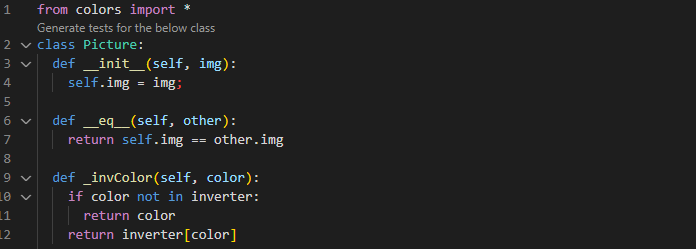
\includegraphics[width=11.2cm]{img/imagen1.png}}}

        \item El método verticalMirror recorre cada fila de la imagen (self.img) y agrega una versión invertida de la fila al resultado (vertical). Luego, devuelve una nueva instancia de Picture con la imagen verticalmente reflejada.    
        \item El método horizontalMirror crea una lista vacía llamada horizontal. Luego, recorre cada fila de la imagen (self.img) y la inserta al principio de la lista horizontal.
        \item[ ]{\raisebox{-0.2\height}{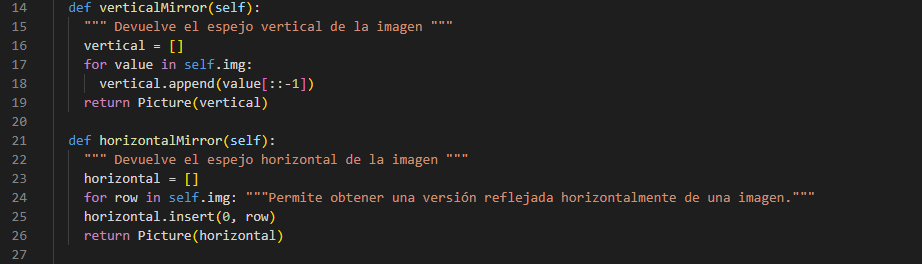
\includegraphics[width=11.2cm]{img/imagen2.png}}}

        \item El método negative recorre cada fila de la imagen (self.img) y crea una nueva fila en la lista negative.
        \item El método join recorre las filas de la imagen actual (self.img) y la imagen pasada como argumento (p.img).
        \item El método up toma otra imagen (p) como argumento y combina verticalmente ambas imágenes.
        \item[ ]{\raisebox{-0.2\height}{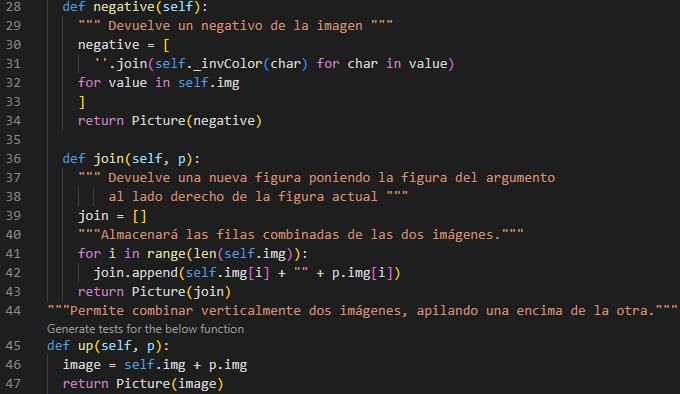
\includegraphics[width=10.2cm]{img/imagen3.png}}}

        \item El método under toma otra imagen p como argumento y devuelve una nueva imagen que combina la imagen actual (self.img) con la imagen p colocada sobre ella.
        \item El método horizontalRepeat toma un valor entero n como argumento y devuelve una nueva imagen que repite la imagen actual (self.img) a su lado n veces.
        \item[ ]{\raisebox{-0.2\height}{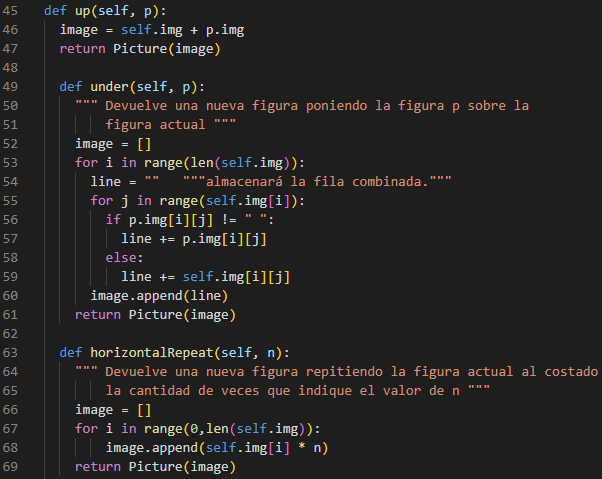
\includegraphics[width=10.2cm]{img/imagen4.png}}}

        \item Este método permite repetir una imagen verticalmente, creando una nueva imagen que contiene múltiples copias de la imagen original una encima de la otra.
         \item[ ]{\raisebox{-0.2\height}{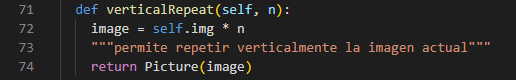
\includegraphics[width=11.2cm]{img/imagen5.png}}}
         
        RESOLVIENDO:

        \item Para resolver los siguientes ejercicios sólo está permitido usar ciclos, condicionales, definición de listas por comprensión, sublistas, map, join, (+), lambda, zip, append, pop, range.
        
        \item Implemente los métodos de la clase Picture. Se recomienda que implemente la clase picture por etapas, probando realizar los dibujos que se muestran en la siguiente preguntas.

        \item Usando únicamente los métodos de los objetos de la clase Picture dibuje las siguientes figuras (invoque a draw):

        Al clonar todos los documentos del GitHub en nuestro repositorio local obtenemos el siguiente 
        resultado.

        Mediante los comandos:
        \item[ ]{\raisebox{-0.2\height}{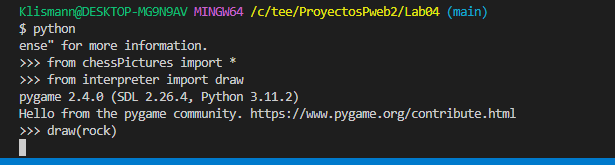
\includegraphics[width=12.2cm]{img/imagen6.png}}}
        
         Obtenemos:
        \item[ ]{\raisebox{-0.2\height}{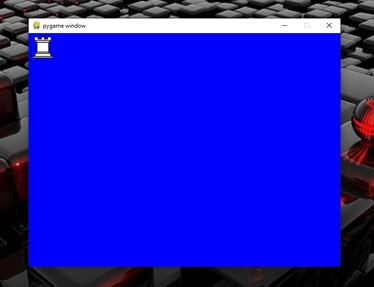
\includegraphics[width=10.2cm]{img/General.png}}}

        Resolviendo: 
        
        Ejercicio2a.
        \item Se crea una figura compuesta por dos filas. En la primera fila, se muestra la imagen knight seguida por su negativo (knight negative).    
        \item[ ]{\raisebox{-0.2\height}{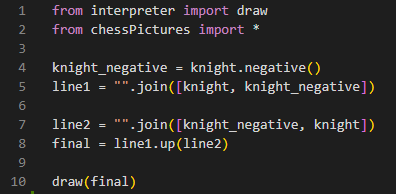
\includegraphics[width=10.2cm]{img/imagen7.png}}}

        Obtenemos:
        \item[ ]{\raisebox{-0.2\height}{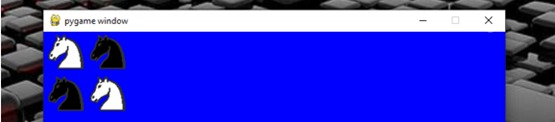
\includegraphics[width=10.2cm]{img/Ejercicio2a.png}}}
        
        Ejercicio2b.
        \item El código crea una figura compuesta por dos filas. En la primera fila, se muestra la imagen knight seguida por su negativo (knightA). En la segunda fila, se muestra la imagen knight espejada verticalmente seguida por la versión espejada verticalmente de knightA. 
        \item[ ]{\raisebox{-0.2\height}{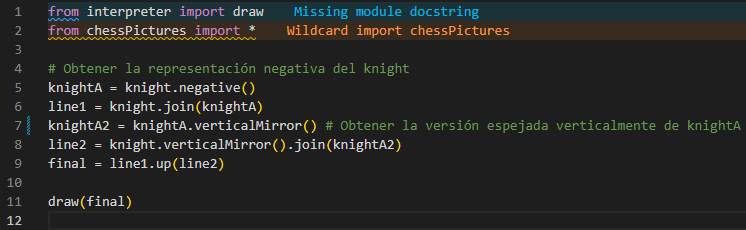
\includegraphics[width=10.2cm]{img/imagen8.png}}}

        Obtenemos:
        \item[ ]{\raisebox{-0.2\height}{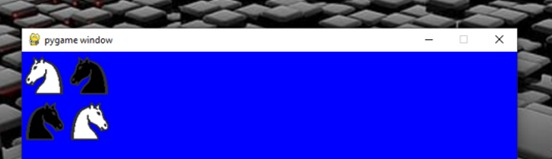
\includegraphics[width=10.2cm]{img/Ejercicio2b.png}}}

        Ejercicio2c.
        \item Se crea una figura compuesta por cuatro copias de la imagen de la reina, donde cada copia se obtiene duplicando la imagen anterior y agregando una nueva copia de la imagen original de la reina.
        \item[ ]{\raisebox{-0.2\height}{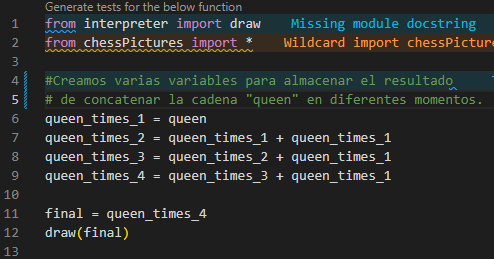
\includegraphics[width=10.2cm]{img/imagen9.png}}}
       
        Obtenemos: 
        \item[ ]{\raisebox{-0.2\height}{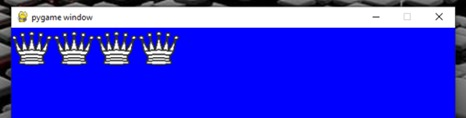
\includegraphics[width=10.2cm]{img/Ejercicio2c.png}}}

        Ejercicio2d.
        \item El código crea una figura compuesta por la concatenación de la imagen square con su negativo.
        \item[ ]{\raisebox{-0.2\height}{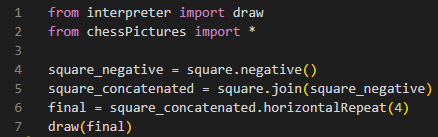
\includegraphics[width=10.2cm]{img/imagen10.png}}}
       
        Obtenemos:
        \item[ ]{\raisebox{-0.2\height}{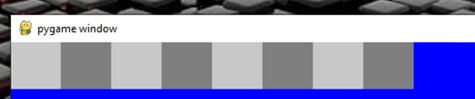
\includegraphics[width=10.2cm]{img/Ejercicio2d.png}}}

        Ejercicio2e.
        \item Se crea una figura compuesta por la concatenación del negativo de la imagen square con la imagen square. Luego, esta figura se repite horizontalmente cuatro veces y se muestra mediante la función draw.
        \item[ ]{\raisebox{-0.2\height}{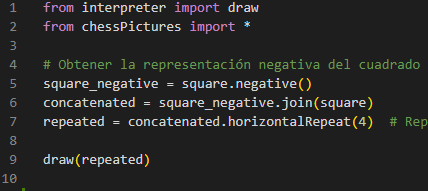
\includegraphics[width=10.2cm]{img/imagen11.png}}}
       
        Obtenemos:
        \item[ ]{\raisebox{-0.2\height}{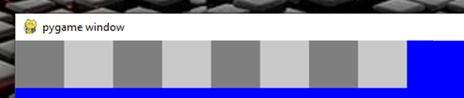
\includegraphics[width=10.2cm]{img/Ejercicio2e.png}}}

        Ejercicio2f.
        \item Se crea una figura compuesta por la concatenación de la imagen square y su negativo, repetida verticalmente dos veces. Luego, esta figura repetida se concatena con su negativo, y finalmente se repite horizontalmente cuatro veces.
        \item[ ]{\raisebox{-0.2\height}{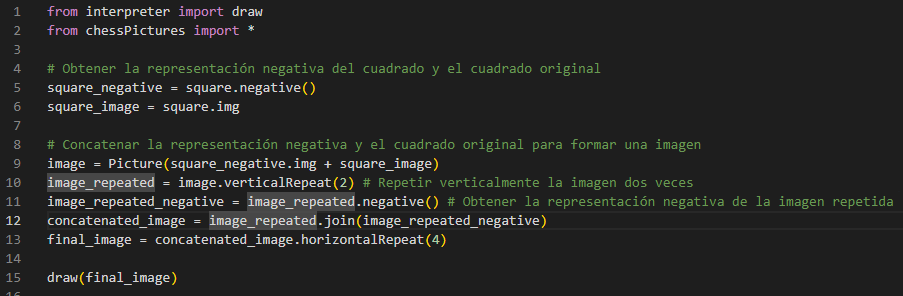
\includegraphics[width=12.2cm]{img/imagen12.png}}}
       
        Obtenemos:
        \item[ ]{\raisebox{-0.2\height}{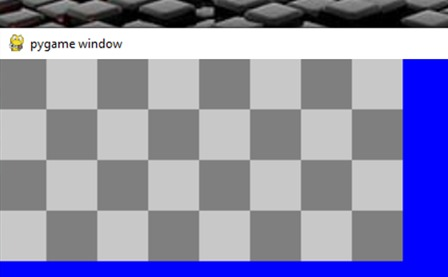
\includegraphics[width=10.2cm]{img/Ejercicio2f.png}}}

        Ejercicio2g.  
        \item Se obtienen los negativos de las figuras.
        \item Se crean las representaciones de las figuras negras en cuadrados claros utilizando el método under y se asignan a las variables correspondientes.
        \item Se crean las representaciones de las figuras negras en cuadrados oscuros utilizando el método under y se asignan a las variables correspondientes.
        \item Se crean las representaciones de las figuras blancas en cuadrados claros.
        \item Se crean las representaciones de las figuras blancas en cuadrados oscuros.
        \item Se crean las representaciones de los reyes y reinas en sus respectivos cuadrados utilizando el método under.
        \item Se crean las filas del tablero uniendo las representaciones de las figuras y cuadrados según la disposición del tablero de ajedrez.
        \item Se llama a la función draw con el argumento tablero para mostrar el tablero de ajedrez resultante.

        \item[ ]{\raisebox{-0.2\height}{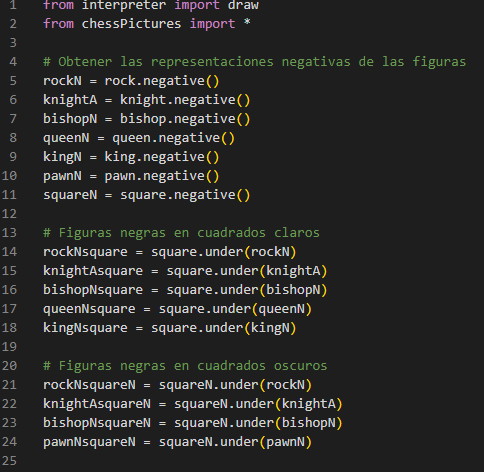
\includegraphics[width=9.8cm]{img/imagen13.png}}}
        \item[ ]{\raisebox{-0.2\height}{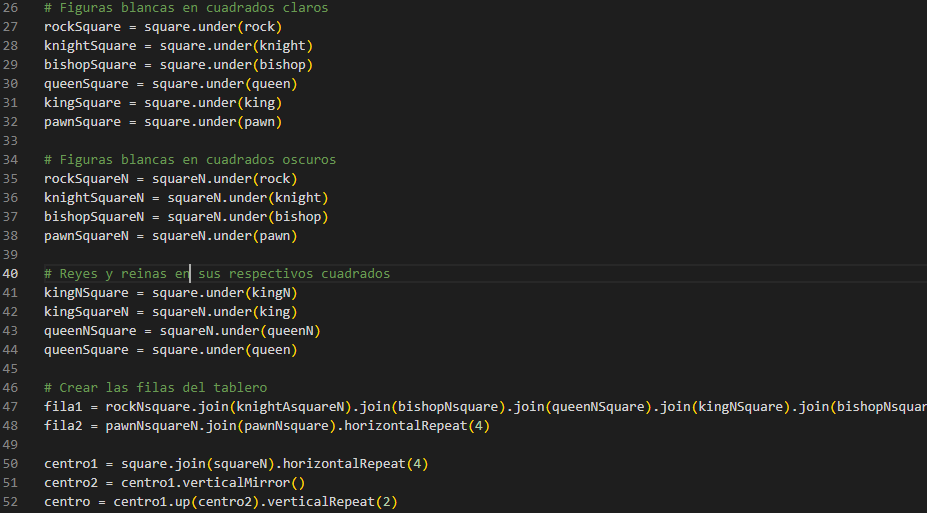
\includegraphics[width=10.2cm]{img/imagen14.png}}} 
        \item[ ]{\raisebox{-0.2\height} {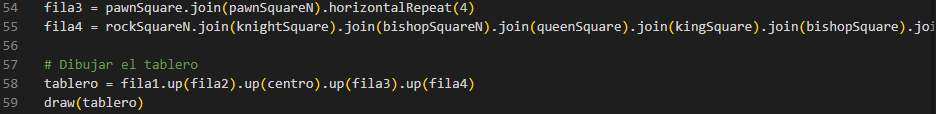
\includegraphics[width=11.2cm]{img/imagen15.png}}}
       
        Obtenemos:
        \item[ ]{\raisebox{-0.2\height}{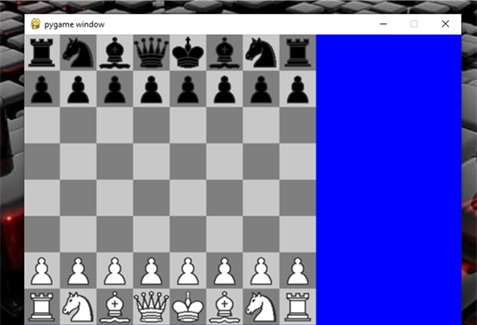
\includegraphics[width=10.2cm]{img/Ejercicio2g.png}}}

        COMMITS
        \item[ ]{\raisebox{-0.2\height}{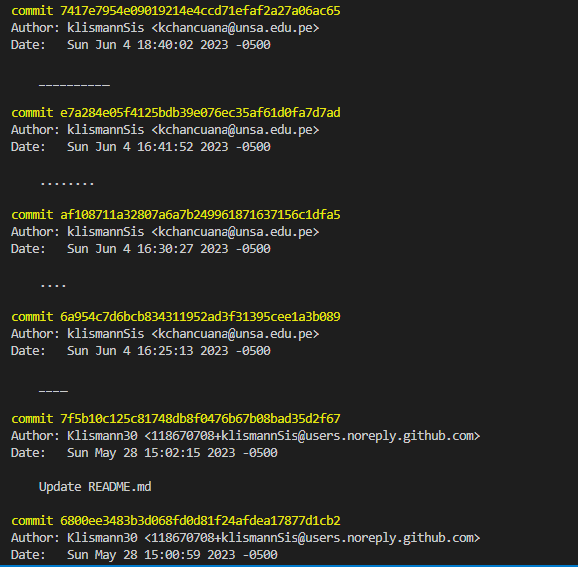
\includegraphics[width=10.2cm]{img/commit1.png}}}
        \item[ ]{\raisebox{-0.2\height}  {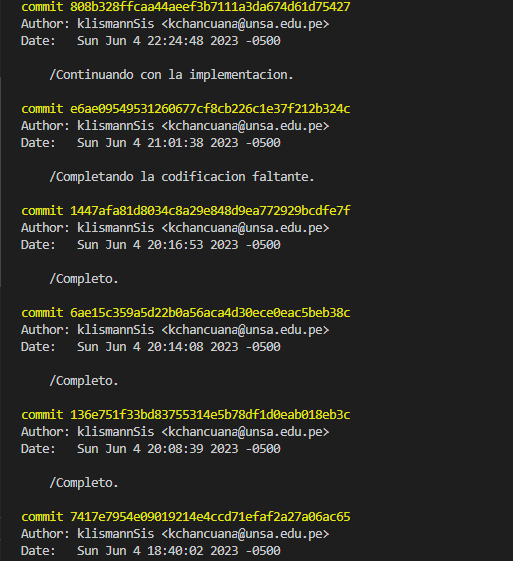
\includegraphics[width=10.2cm]{img/commit2.png}}}
        \item[ ]{\raisebox{-0.2\height}{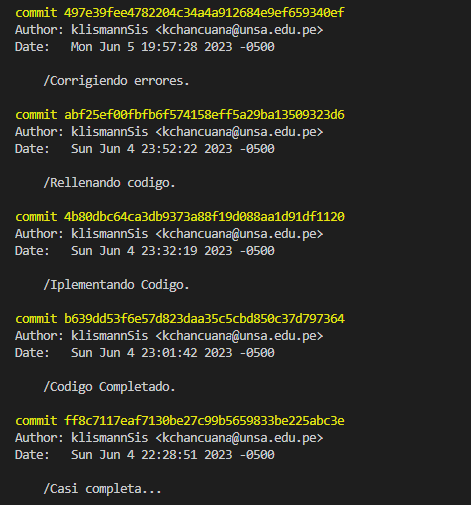
\includegraphics[width=10.2cm]{img/commit3.png}}}
        \item[ ]{\raisebox{-0.2\height}{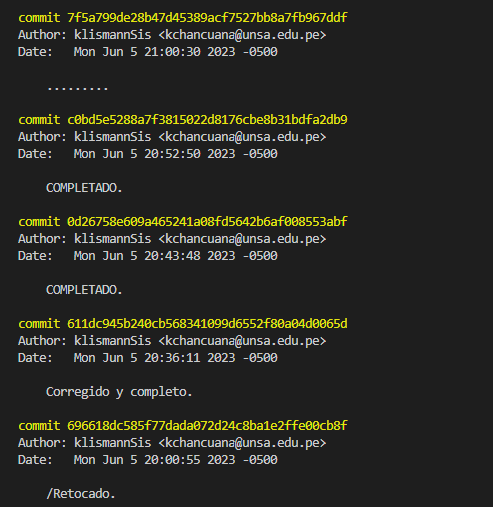
\includegraphics[width=10.2cm]{img/commit4.png}}}
        \item[ ]{\raisebox{-0.2\height}{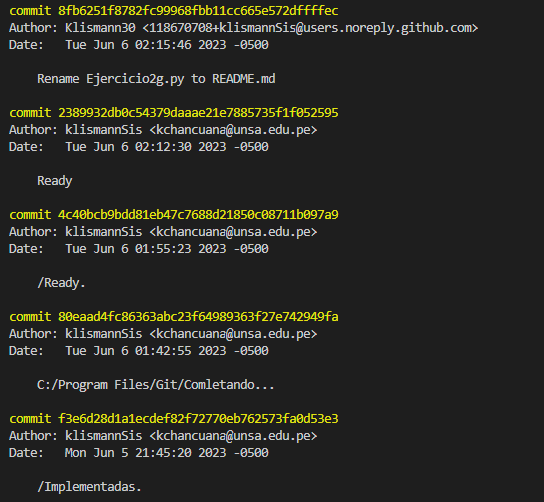
\includegraphics[width=12.2cm]{img/commit5.png}}}
        \item[ ]{\raisebox{-0.2\height}{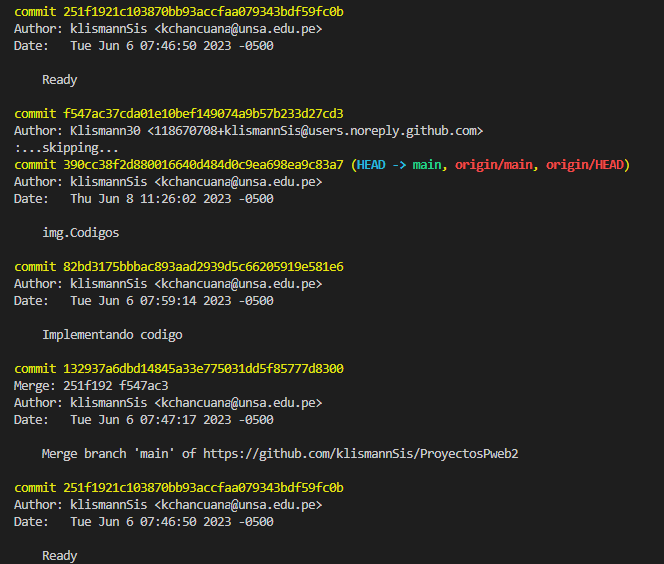
\includegraphics[width=12.2cm]{img/commit6.png}}}
        \item[ ]{\raisebox{-0.2\height}{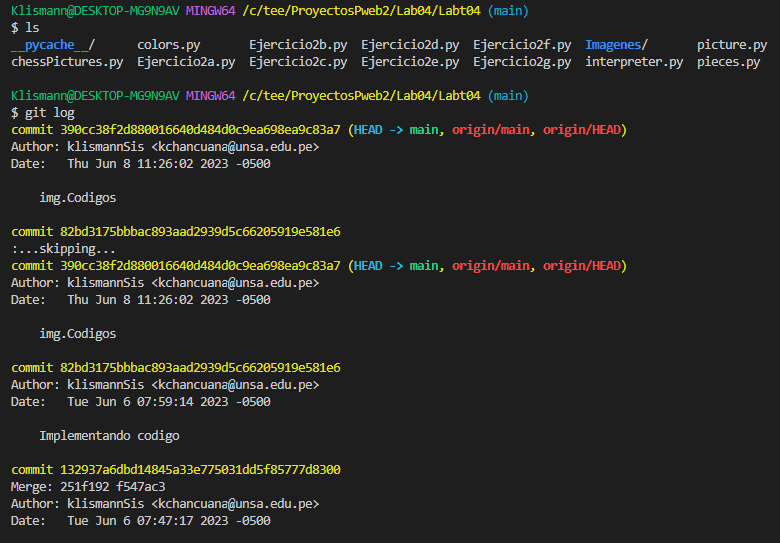
\includegraphics[width=12.2cm]{img/commit7.png}}}
           
	\end{itemize}
		
	\section{Equipos, materiales y temas utilizados}
	\begin{itemize}
		\item Sistema Operativo Ubuntu GNU Linux 23 lunar 64 bits Kernell 6.2.
		\item VIM 9.0.
		\item Python 3.11.2.
		\item Git 2.39.2.
		\item Cuenta en GitHub con el correo institucional.
		\item Programación Orientada a Objetos.
		\item Algoritmo de ordenamiento por inserción	
	\end{itemize}
	
	\section{URL de Repositorio Github}
	\begin{itemize}
		\item URL del Repositorio GitHub para clonar o recuperar.
		\item \url{https://github.com/rescobedoq/pw2.git}
		\item URL para el laboratorio 01 en el Repositorio GitHub.
		\item \url{https://github.com/rescobedoq/pw2/tree/main/labs/lab04}
	\end{itemize}
		
	\begin{itemize}	
		\item Link del repositorio github
        \item \url{https://github.com/klismannSis/ProyectosPweb2/tree/main/Lab04}
	\end{itemize}

\section{Cuestionario}

	\begin{document}
    \item ¿Qué son los archivos *.pyc?
    \item  
    los archivos ".pyc" son archivos de código byte compilado en Python que se   utilizan para acelerar la carga y ejecución de programas, así como para     proteger el código fuente original.

    \item
    \item ¿Para qué sirve el directorio pycache? 
    \item
    
    Los archivos ".pyc" en Python son archivos que contienen el código compilado de un programa. Cuando 
    un programa en Python se ejecuta, el intérprete traduce el código fuente a un formato intermedio 
    llamado bytecode. Este bytecode se guarda en archivos ".pyc" para permitir su reutilización en 
    ejecuciones futuras del programa.
    
    \item
    \item ¿Cuáles son los usos y lo que representa el subguión en Python?
    \item
    
        - Un guión bajo () (class)
        Se utiliza para evitar conflictos con palabras clave o elementos relacionados.
        
        - Un guión bajo (variable)
        En este caso indica que el nombre que sigue al guion es una clase, función, método o variable.  
        - Un doble guión bajo () (Klismann)
        
        Cualquier mombre de la forma anonimo se sustituye por NombreClase anonimo.
        - Un doble guion bajo () ( casa ).
        Se utiliza para indicar métodos específicos conocidos como métodos mágicos, init, file.
        Su objetivo es evitar conflictos entre los métodos mágicos y algún método definido por nosotros.
        
        
        
   \section{Conclusion} 
   El código de tablero de ajedrez demuestra el uso de diferentes conceptos y técnicas de 
   programación. Las clases y los métodos se utilizan para organizar y organizar el código. Además, se 
   controlan imágenes y se colocan aplicaciones para combinar y repetir los procesos para construir un 
   tablero completo. Sin embargo, el código demuestra el uso de programación orientada a objetos, 
   operaciones de visualización de datos y el uso de lógica de bucle para lograr el resultado deseado.

    
\section{\textcolor{red}{Rúbricas}}
	
	\subsection{\textcolor{red}{Entregable Informe}}
	\begin{table}[H]
		\caption{Tipo de Informe}
		\setlength{\tabcolsep}{0.5em} % for the horizontal padding
		{\renewcommand{\arraystretch}{1.5}% for the vertical padding
		\begin{tabular}{|p{3cm}|p{12cm}|}
			\hline
			\multicolumn{2}{|c|}{\textbf{\textcolor{red}{Informe}}}  \\
			\hline 
			\textbf{\textcolor{red}{Latex}} & \textcolor{blue}{En conclusion este informe esta editado en latex y en formato PDF.}   \\ 
			\hline 
			
			
		\end{tabular}
	}
	\end{table}

\section{Referencias}
\begin{itemize}			
	\item \url{https://www.w3schools.com/python/python_reference.asp}
	\item \url{https://docs.python.org/3/tutorial/}
\end{itemize}	
	
%\clearpage
%\bibliographystyle{apalike}
%\bibliographystyle{IEEEtranN}
%\bibliography{bibliography}
			
\end{document}
	
